\begin{enumerate}

\item[a)]Definimos las entradas 13 (tarea inicial), 14 (tarea idle), 15-22 (tareas jugador 1), 23-30 (tareas jugador 2) de la GDT
A estas entradas se les asigna tipo 9 (Execute-Only,accessed), base 0, presente 1 y DPL 0. El límite se establece en {\tt 0x67} para que sea mayor al tamaño de una TSS. La Figura \ref{fig:gdt2} muestra el estado de la GDT luego de agregar estas entradas.

\begin{figure}
  \centering
    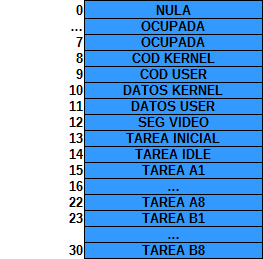
\includegraphics[width=0.50\textwidth]{imagenes/gdtfinal.png}
  \caption{Estado final de la GDT}
  \label{fig:gdt final}
\end{figure}
 \FloatBarrier

\item[b)]Para completar la TSS de la tarea Idle hacemos uso de la función {\tt tss\_inicializar\_tarea\_idle}, la cual se encarga de asignar los segmentos de datos del kernel a los campos GS, FS, DS, SS, ES y poner el segmento de código de kernel en el campo CS. A su vez, completa ESP y EBP con la dirección del stack del kernel y se ocupa de que comparta el cr3 con el kernel. Por último, el EIP será {\tt 0x16000}, el campo EFLAGS se completa con {\tt 0x202} (para habilitar las interrupciones), el IOMAP con {\tt 0xFFFF} y el resto se deja en 0.

\item[c)] La función {\tt tss\_inicializar\_tareas\_piratas} toma como parámetro un puntero a tss y se ocupa de llenar sus campos. Los campos ES, SS, DS, FS y GS se completan con el segmento de datos de usuario, y el campo CS se completa con el segmento de código de usuario. ESP y EBP quedan seteados en {\tt 0x401000-12} y {\tt 0x401000-4} respectivamente, el campo EFLAGS en {\tt 0x202}, el CR3 en 0 (se le asignará un cr3 al momento de lanzar el pirata correspondiente utilizando la función {\tt mmu_inicializar_dir_tarea}), se pedirá una página nueva para el ESP0, SS0 se completa con segmento de datos kernel, IOMAP con {\tt 0xffff} y el resto con 0. 

\item[d)] En la rutina {\tt tss\_inicializar} pedimos una página libre para la tss de la tarea inical y asignamos la dirección obtenida en el campo {\it base} de la entrada correspondiente a esta tarea en la GDT.

\item[e)] En la rutina {\tt tss\_inicializar} completamos la entrada de la GDT perteneciente a la tarea Idle, completando el campo {\it base} con la dirección correspondiente a la misma.

\item[f)]Para pasar a la tarea IDLE primero se carga la tarea inicial en {\tt kernel.asm}, haciendo uso de la instruccion {\tt ltr} y de la dirección del segmento de la tss inicial. Una vez cargada la tarea inicial, se ejecuta un {\tt jmp} a la etiqueta seg_tss_idle, que corresponde al segmento de la tss Idle.

\begin{lstlisting}[frame=single]
define selector_Inicial 0x0068 ;0000000001101011
define selector_Idle 0x070 ;0000 0000 0111 0011

...

; Cargar tarea inicial
mov ax, selector_Inicial
ltr ax

; Saltar a la primera tarea: Idle
jmp selector_Idle:0

...
\end{lstlisting}

\item[g)]Se modifica el comportamiento de la rutina de atención de la interrupción {\tt 0x46} de la siguiente manera. Se pasan los 2 parámetros a {\tt game\_syscall\_manejar} y se la ejecuta. Luego de haber terminado {\tt game\_syscall\_manejar} se encargará de saltar a la tarea idle. 

La función {\tt game\_syscall\_manejar} determina en base al primer parámetro tomado si se quiere ejecutar un syscall mover, cavar o posición y llama a {\tt game\_syscall\_pirata\_mover}, {\tt game\_syscall\_cavar} o {\tt game\_syscall\_pirata\_posicion} según corresponda. Analizaremos por separado los 3 casos:
\begin{itemize}

\item Caso mover: Según el jugador y el índice de la tarea que se encuentren jugando en el momento se busca el pirata que corresponde en el arreglo de piratas del jugador (piratasA o piratasB) así como también el arreglo de posiciones visitadas del jugador (visitadasA o visitadasB). Una vez obtenidos estos, se busca la posición actual del pirata y se cheque si el movimiento que desea realizar es válido o no (en caso de que no lo sea se llama a la función {\tt game\_matar\_pirata\_interrupt}, en caso de ser válido se calcula la posición destino y la dirección virtual asociada a esa posición, se busca el cr3 de la tarea en su tss y se actualiza la posición del pirata. En el caso de que el pirata fuera un minero se llama a {\tt revisar\_mapeadas} que como indica su nombre, revisa si la posición virtual destino ya habia sido explorada, en caso de que no lo fuera, se mata a la tarea.
Pasado este punto se llama a {\tt copiar\_codigo} con el cr3, la posición virtual destino, la posición virtual asociada a la posición anterior y las componentes x e y de la posición destino.
En caso de que estuvieramos hablando de un explorador, este mapea las nuevas direcciones exploradas a todas las tareas del jugador, actualiza el arreglo de visitadas y el indice de la última posición válida del arreglo y pasa a buscar botines. Para buscar los botines, se revisa si hay algun elemento en el arreglo de botines que entre en el rango recientemente explorado y contenga monedas, de ser así, se lo pinta en el mapa y se llama a {\tt game\_jugador\_lanzar\_pirata} que lanzara una tarea pirata para el jugador, de tipo minero, y con la posición del botín descubierto. Para finalizar, se llama a {\tt screen\_pintar\_pirata} con un puntero al jugador y al pirata, y se lo pinta con los colores correspondientes en el mapa.


\item Caso cavar: Según el jugador y el índice de la tarea que se encuentran jugando en el momento se busca el pirata que corresponda y se obtiene su posición. Con esta posición se recorre el arreglo de botines buscando alguno que encaje en la posición del minero. En caso de que el botin ya no tenga mas monedas, se mata a la tarea. Caso contrario, se aumenta el puntaje del jugador en 1, se actualiza el puntaje en pantalla y se decrementa la cantidad de monedas en el botín en 1.

\item Caso posición: Según el jugador que se encuentra jugando, y el parámetro de la función, se va al arreglo de piratas correspondiente al jugador y segun el parámetro se busca el pirata cuyo índice corresponda (en caso de ser 0-8) o el pirata actual (en caso de ser -1). Una vez obtenida la posición del pirata, se crea una variable resultado, se le suma la componente y, se shiftea 8 lugares y se le suma la componente x. Se termina retornando dicha variable.
\end{itemize}
\item[h)]Para este apartado hicimos algo más que lo pedido por el enunciado. Probamos lanzar una tarea explorador a través los siguientes pasos: llamar a {\tt inic_game} (función que se encarga de inicializar las variables globales del juego como los jugadores con sus respectivos puertos, 0 tareas activas, etc y todas las tareas piratas correspondientes a cada jugador como muertas y con sus respectivos indices, entre otras cosas), luego, mediante {\tt tss_inicializar} realizamos lo concerniente a la tss de las tareas (dejando lugar para un cr3 que se creara luego), y para finalizar ya dentro del juego presionamos la tecla RSHIFT (cual shift se presiona resulta indiferente para los efectos de la prueba). Presionando RSHIFT se llama a {\tt game_lanzar_pirata} que se encarga de inicializar el mapa de memoria de la tarea, copiar su codigo en el mapa y completar su campo posicion, además de mostrarla en el mapa de juego. Por último se procede a correr esa tarea previamente lanzada.

\end{enumerate}